\documentclass[border=4pt,crop=true]{standalone}
\usepackage{pgfplots}
\pgfplotsset{compat=1.18}

% Shockley: i = I_s (exp(v/V_T) - 1), plot i in mA
\def\Is{1e-14}
\def\Vt{0.025}

\begin{document}
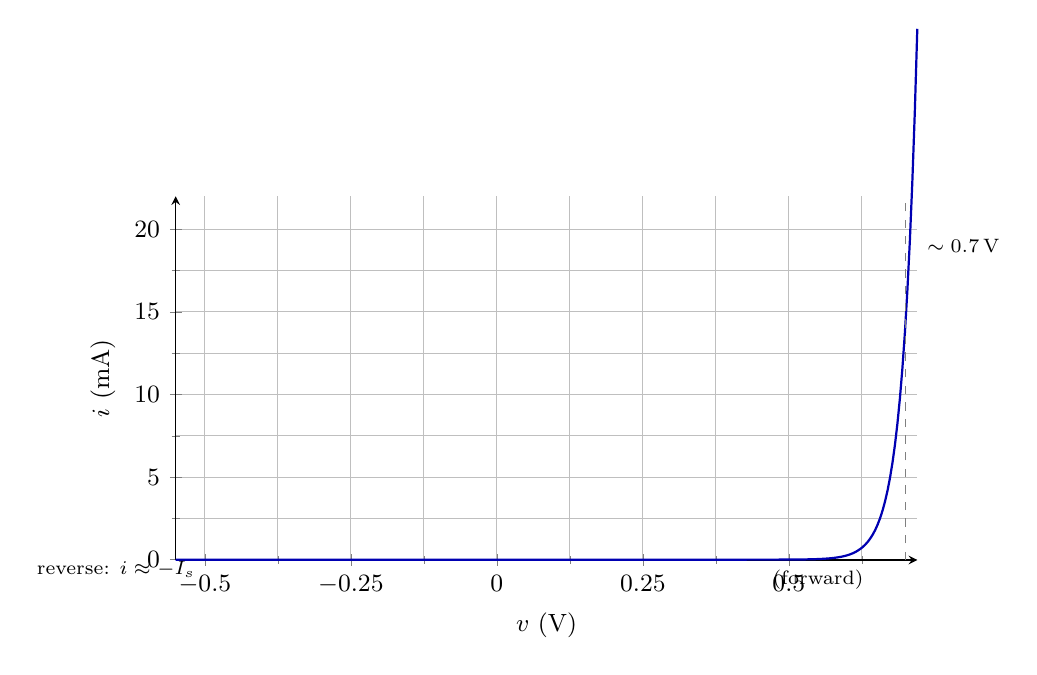
\begin{tikzpicture}
  \begin{axis}[
    width=11cm,
    height=6.2cm,
    xmin=-0.55,
    xmax=0.72,
    ymin=-0.02,
    ymax=22,
    axis lines=left,
    xlabel={$v$ (V)},
    ylabel={$i$ (mA)},
    xtick={-0.5,-0.25,0,0.25,0.5,0.75},
    ytick={0,5,10,15,20},
    grid=both,
    minor tick num=1,
    tick label style={font=\small},
    label style={font=\small},
    every axis plot/.append style={thick},
    clip=false,
  ]
    \addplot[blue!70!black, domain=-0.55:0.72, samples=300]
      {1000*\Is*(exp(x/\Vt) - 1)};
    \draw[dashed, gray] (axis cs:0.7,-0.02) -- (axis cs:0.7,22);
    \node[font=\scriptsize, anchor=south west] at (axis cs:0.72,18)
      {$\sim 0.7\,\mathrm{V}$};
    \node[font=\scriptsize, anchor=north] at (axis cs:0.55,-0.02)
      {(forward)};
    \node[font=\scriptsize, anchor=north east] at (axis cs:-0.5,0.5)
      {reverse: $i\approx -I_s$};
  \end{axis}
\end{tikzpicture}
\end{document}
